\documentclass[12pt, a4papre]{article}
\usepackage[catalan]{babel}
\usepackage[unicode]{hyperref}
\usepackage{amsmath}
\usepackage{amssymb}
\usepackage{amsthm}
\usepackage{xifthen}
\usepackage{listings}
\usepackage{float}
\usepackage{siunitx}
\usepackage{graphicx}
\usepackage{indentfirst}

\newcommand{\norm}[1]{\lvert #1 \rvert}
\graphicspath{ {./Images/} }

\hypersetup{
    colorlinks = true,
    linkcolor = blue
}

\author{Daniel Vilardell}
\title{Previ practica 3}
\date{}

\begin{document}
	\maketitle
	
	\textbf{Qüestió 1.1:} Ho podem analitzar com un divisor de tensió. Veiem primer que si considerem $z_1$ el condensador i resistencia en seria i $z_2$ el condensador i resistencia en paralel tenim la seguent igualtat.
	
	\[
		z_1 = \frac{1+RCs}{Cs} \qquad z_2 = \frac{R}{1+RCs}
	\]
	
	Per tant aplicant la formula de un divisor de tensió tenim que
	
	\[
		\frac{V_o}{V_i} = \frac{\frac{R}{1+RCs}}{\frac{1+RCs}{Cs} + \frac{R}{1+RCs}} = \frac{RCs}{(1+RCs)^2+RCs} = 
		\frac{RCs}{1+3RCs+(RCs)^2}=
	\]
	\[
		= \frac{\frac{s}{RC}}{s^2+\frac{3s}{RC}+\frac{1}{(RC)^2}}
	\]
	
	\textbf{Qüestió 1.2:} Tenint en conte que $H(s) = \frac{A\cdot w_o\cdot s}{s^2+\frac{w_o}{Q}s+w_o^2}$ obtenim que
	
	\begin{itemize}
		\item $w_o = \frac{1}{RC}$
		\item $Q = \frac{1}{3}$
		\item $A = 1$
	\end{itemize}
	
	El guany a la frequencia central serà
	
	\[
		H(jw_o) = \frac{Aw_o^2j}{(jwo)^2+\frac{w_o}{Q}jw_o+w_o^2} = QA \implies G = |QA| = \frac{1}{3}
	\]
	
	\textbf{Qüestió 1.3:} Si tenim que $w_o = 2\pi f_o = \frac{1}{RC}$ podem deduir que la resistencia que ens falta trobar tindrà el valor de 
	
	\[
		R = \frac{1}{2\pi f_oC} = \frac{1}{2\pi 10^3\cdot 10 \cdot 10^{-9}} = 15.8kHz
	\]
	
	\textbf{Qüestió 2.1:} Sabent que $T(s) = af$ obtenim que
	
	\[
		T(s) = H(s)f_R = \frac{\frac{1}{RC}f_R s}{s^2+\frac{3s}{RC}+\frac{1}{(RC)^2}} = \frac{2000\pi f_Rs}{s^2+6000\pi s+4\pi^210^6}
	\]
	
	$T(s)$ te un zero a $s=0$ i dos pols, un a $s=-2.4\cdot 10^3$ i l'altre a $s=-16.47\cdot 10^3$ 
	
	Tenim que $T(s) = -1$ per tant
	
	\[
		T(s) = k\frac{s}{s^2+\frac{3s}{RC}+\frac{1}{(RC)^2}} = -1 \implies s^2+\frac{3}{RC}s+\frac{1}{(RC)^2}+ks = 0
	\] 
	\[
		Routh \implies \frac{3}{RC}+k = 0 \implies k = \frac{-3}{RC}
	\]
	
	Suposem primer que $f_R < 0$ aleshores tenim que 
	
	\begin{figure}[H]
		\begin{center}
		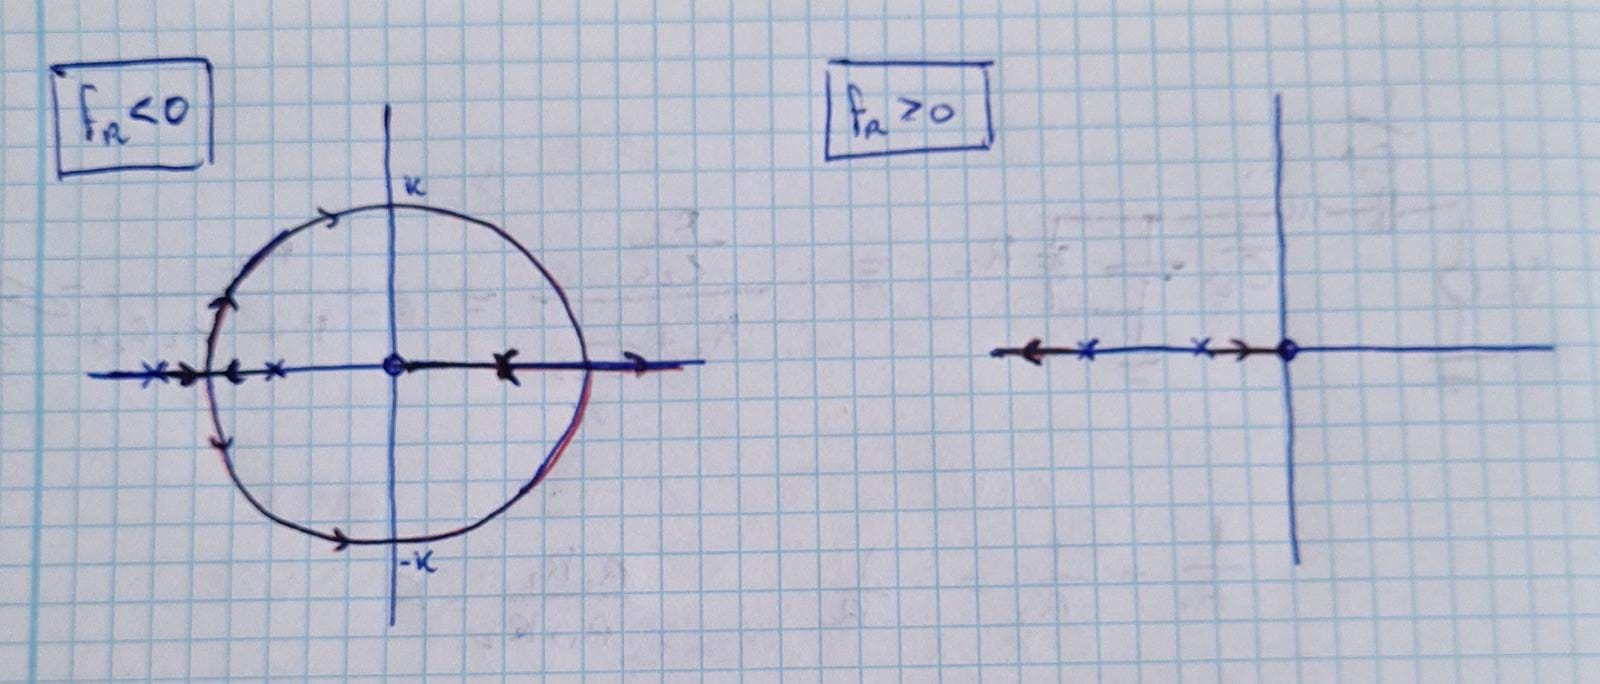
\includegraphics[width=100mm]{img_p_3_1.jpeg}
		\caption{Lloc geometric de les arrels}
		\end{center}
	\end{figure}
	
	Observem que el circuit no sera estable per tot $f_R$. Oscilara si $k = \frac{-3}{RC}$, per tant sera estable per els valors
	
	\[
		k = \frac{f_R}{RC} > \frac{-3}{RC} \iff -3 < f_R < 0
	\]	
	
	\textbf{Qüestió 2.2:} Hem vist a teoria que $H_R(s) = \frac{V_o(s)}{V_i(s)}  = \frac{a(s)}{1+T(s)}$. Per tant tenim que
	
	\[
		H_R(s) = \frac{H(s)}{1+T(s)} = \frac{\frac{\frac{s}{RC}}{s^2+\frac{3s}{RC}+\frac{1}{(RC)^2}}}{1+ \frac{\frac{1}{RC}f_R s}{s^2+\frac{3s}{RC}+\frac{1}{(RC)^2}}} = \frac{\frac{s}{RC}}{s^2+\left(\frac{3}{RC}+\frac{f_R}{RC}\right)s+\frac{1}{(RC)^2}}
	\]
	
	D'aquí podem obtenir que 
	
	\[
		w_o = \frac{1}{RC} \implies \frac{w_o}{Q} = \frac{3+f_R}{RC} = (3+f_R)w_o \implies Q = \frac{1}{3+f_R}
	\]
	
	Si busquem un factor de qualitat $Q=5$ necessitem que $5 = \frac{1}{3+f_R} \implies f_R = -2.8$
	
	Si busquem un factor de qualitat $Q=10$ necessitem que $10 = \frac{1}{3+f_R} \implies f_R = -2.9$
	
	El circuit com hem vist al apartat 2.1 es torna inestable sempre que $f_R < -3$, per tant si $Q = 5$ o $Q = 10$ el circuit tindria una $f_R > -3$ i per tant seria estable.
	
	Si $Q = 5$ aleshores tindriem els pols a $s = -200\pi \pm 6.26j$ i si $Q = 10$ els pols serien $s = -100\pi \pm 6.28j$
	
	\begin{figure}[H]
		\begin{center}
		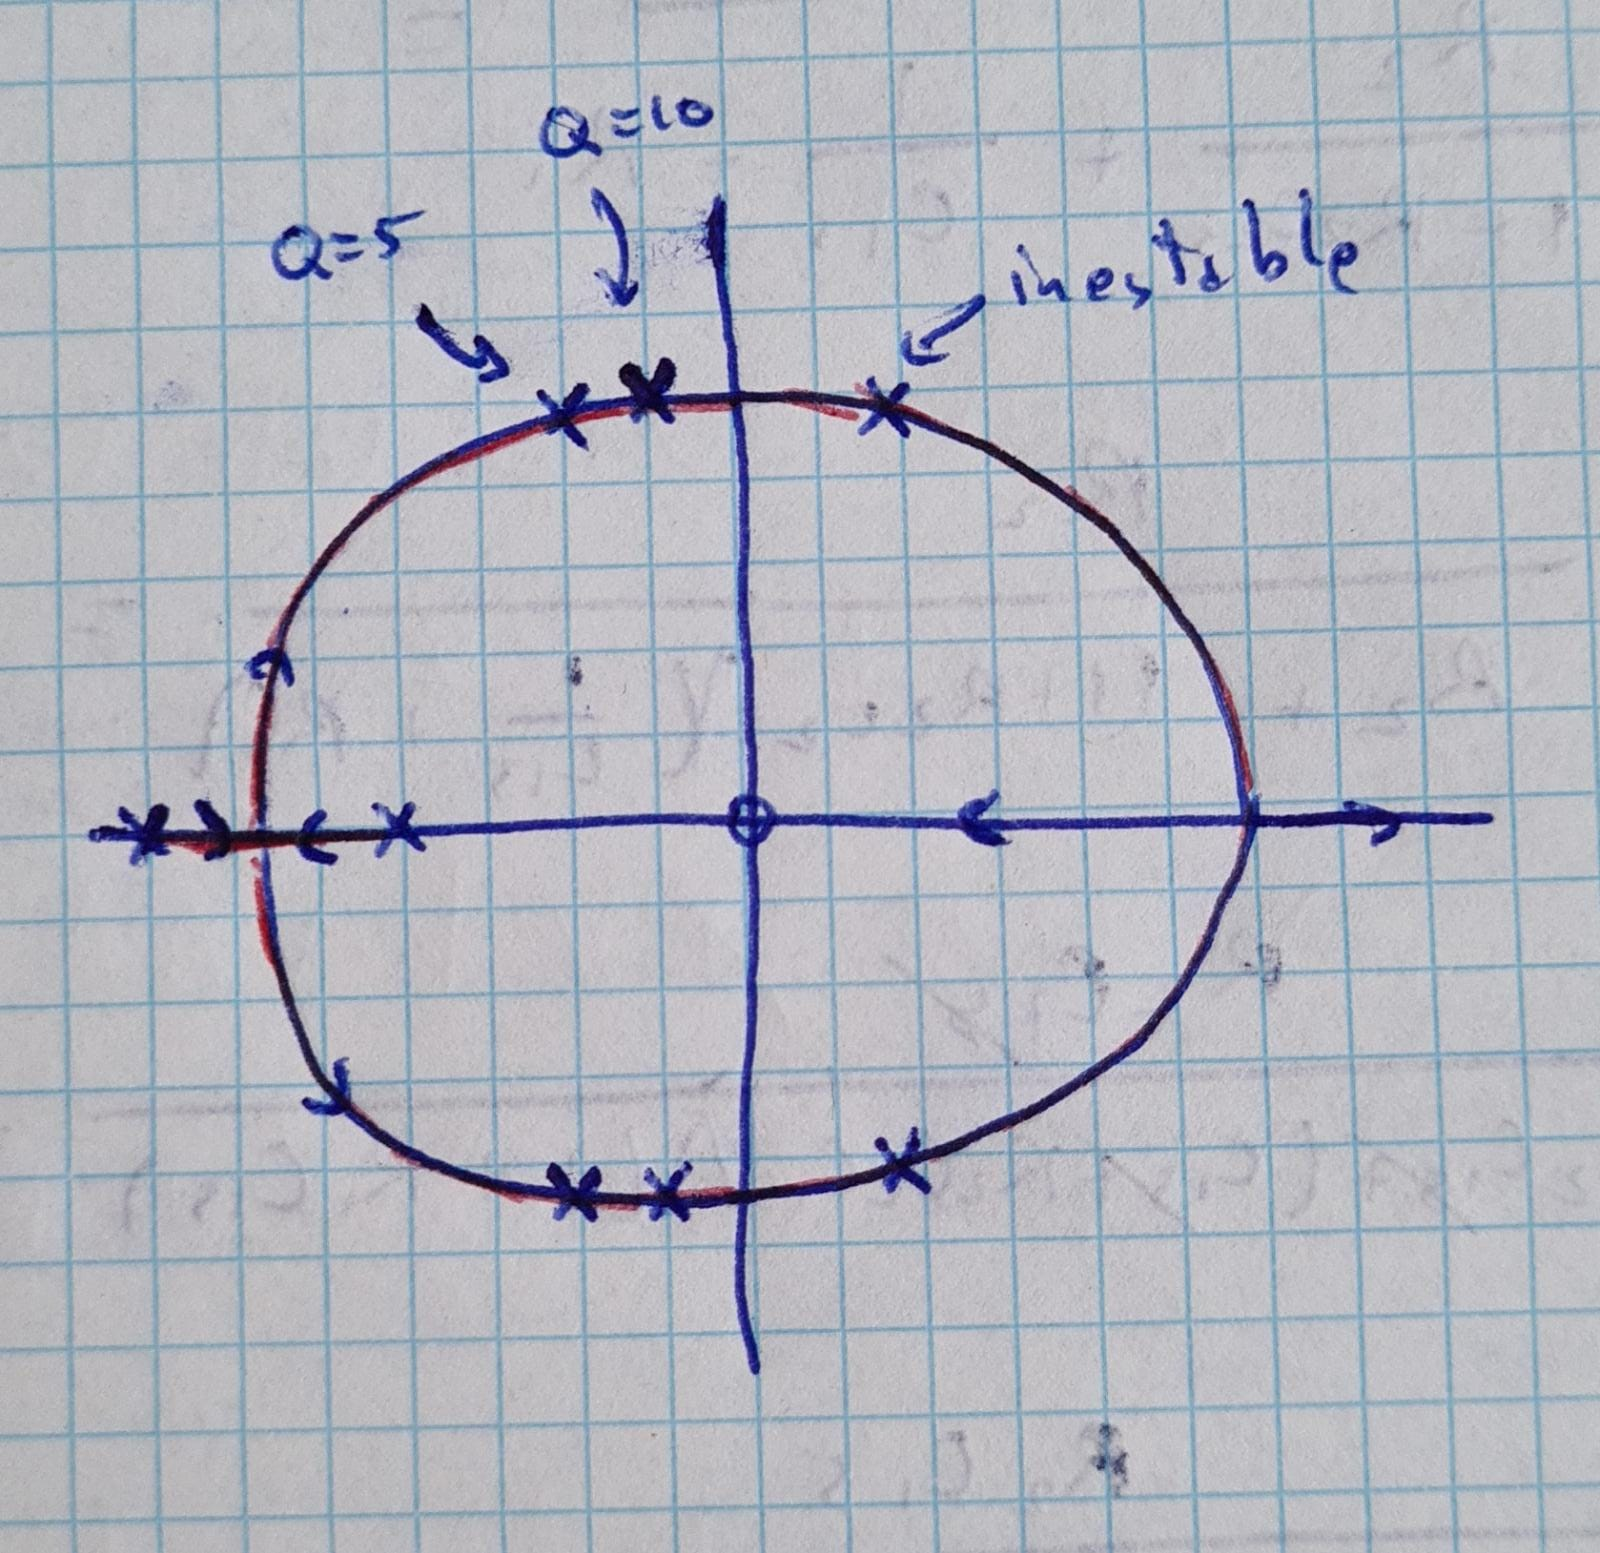
\includegraphics[width=70mm]{img_p_3_2.jpeg}
		\caption{Lloc geometric de les arrels}
		\end{center}
	\end{figure}
	
	\textbf{Qüestió 3.1:} Busquem com es relaciona $V_x$ amb $V_i$ i $V_o$.
	
	\[
		\frac{V_o-V_i}{R_a} +\frac{V_o-V_x}{R_f} = 0 \implies V_x = \frac{R_f}{R_a}V_i +(1+\frac{R_f}{R_a})V_{o}
	\]
	
	La relació entre $V_o$ i $V_x$ la hem obtingut a la questio 1.1 i es $H(s)$. Per tant tenim que el diagrama de fluxe es el següent.
	
	\begin{figure}[H]
		\begin{center}
		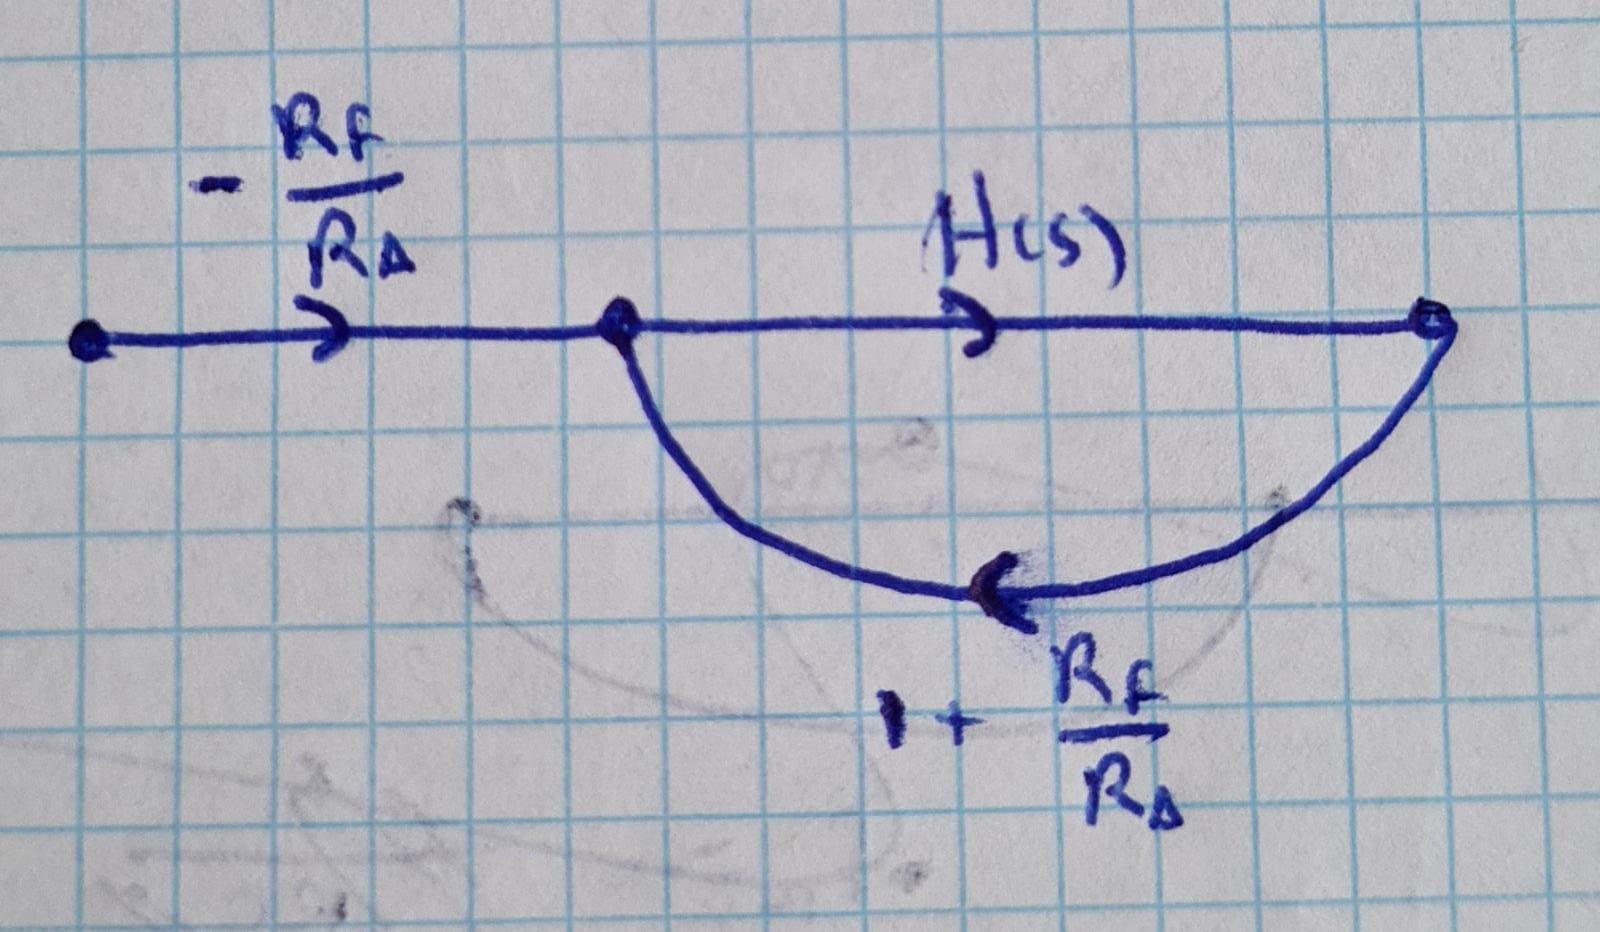
\includegraphics[width=70mm]{img_p_3_3.jpeg}
		\caption{Diagrama de fluxe del circuit}
		\end{center}
	\end{figure}
	
	D'aquí obtenim que $\alpha = \frac{R_f}{R_a}$ i que $f_R = -(1+\frac{R_f}{R_a})$.
	
	Si ara suposem que $R_a = 10k\si{\ohm}$ busquem els valors de $R_a$ per a que $Q = 5$ i $Q = 10$.
	
	\[
		Q = 5 \implies f_R = -2.8 = -(1+\frac{R_f}{R_a}) \implies R_f = 1.8R_a = 18k\si{\ohm}
	\]
	
	\[
		Q = 10 \implies f_R = -2.9 = -(1+\frac{R_f}{R_a}) \implies R_f = 1.9R_a = 19k\si{\ohm}
	\]
	
\end{document}




